\subsection{Columbia Game Corpus}

\begin{figure}
\centering
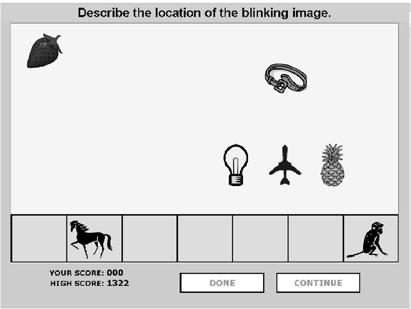
\includegraphics[width=10cm]{images/columbia_games.jpg}
\caption{Juego del Columbia Games}
\end{figure}

Nuestro corpus consiste en doce conversaciones diádicas (i.e., con dos participantes) entre trece personas distintas. En cada sesión, se sentó a dos participantes (quienes no se conocían previamente) en una cabina profesional de grabación, cara a cara a ambos lados de una mesa, y con una cortina opaca colgando entre ellos para evitar la comunicación visual.

Los participantes contaron con sendas computadoras portátiles conectadas entre sí, en las cuales jugaron una serie de juegos simples que requerían de comunicación verbal. Por ejemplo, en uno de tales juegos, ambas computadoras muestran un tablero con varios objetos (Figura 1), todos en la misma posición excepto por uno, el objetivo, que aparece en un lugar distinto en cada computadora.

Uno de los jugadores, para quien el objetivo aparece titilando, debe entonces describir la ubicación exacta del mismo usando los
otros elementos como referencia, de modo que el otro jugador pueda mover su propia instancia del objetivo a la posición correcta. Al terminar cada juego, se otorga un puntaje según la precisión de la tarea realizada.

Las grabaciones se hicieron en 44 kHz, 16 bits con un canal separado para cada hablante; luego fueron guardadas en 16 kHz para el presente estudio. Cada sesión duró aproximadamente 45 minutos, totalizando 9 horas de diálogos, 70.259 palabras (2.037 únicas) para todo el cuerpo de datos.
